\chapter{Results}\label{chap:results}
 \section{Different performance metrics of Model}
The network is very simple with following parameters.
 \begin{itemize}
     \item \textit{Activation:} Relu
     \item \textit{Optimizer:} Adam
     \item \textit{Filter size:} $3 \times 3 $
     \item  25 epochs and 200 batch-size
     \item \textit{Dataset:} MNIST
\end{itemize}
 Now let us look at the variation of accuracy and loss during the training.
 
\begin{figure}[h]
    \centering
    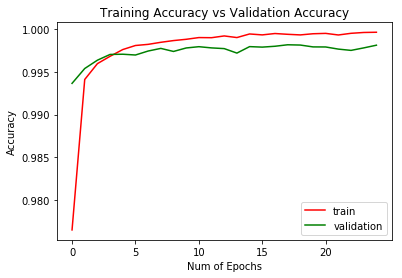
\includegraphics[width=0.6\textwidth]{thesis_template/images/accmnist.png}
    \caption{\small Accuracy of the model during training for 25 epochs on MNIST}
    \label{}
    \end{figure} 
    
\noindent As we can see in the graph the model converged with less number of epochs and has achieved the accuracy of 99.8\% on both train and validation sets. On test set it has achieved accuracy of 99.4\%.
    \begin{figure}[h]
    \centering
    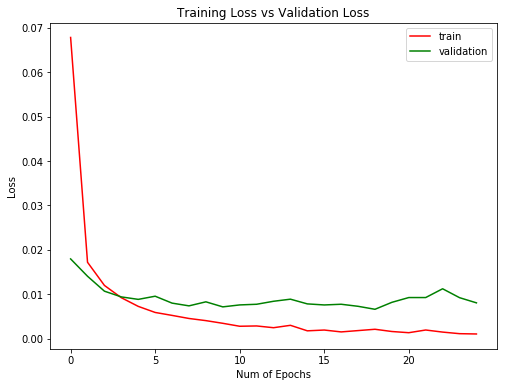
\includegraphics[width=0.5\textwidth]{thesis_template/images/lossmnist.png}
    \caption{\small Variation of loss of the model during training for 25 epochs on MNIST}
    \label{}
    \end{figure}    

\noindent The loss of the model is 0.001\% on train set and 0.006\% on validation set.

\begin{figure}[h]
    \centering
    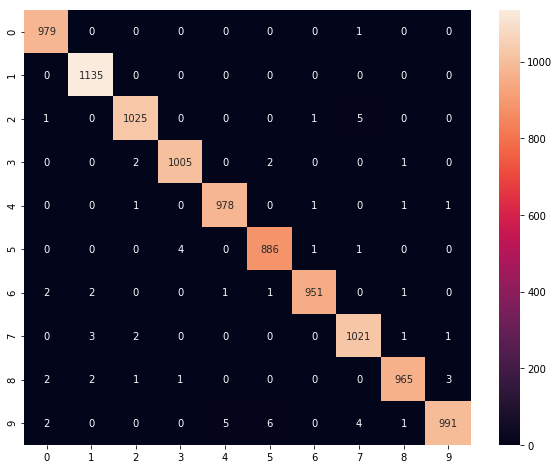
\includegraphics[width=0.6\textwidth]{thesis_template/images/confmatrix.png}
    \caption{\small Confusion-matrix for a model trained for 25 epochs on MNIST}
    \label{}
    \end{figure}

\noindent The image represents the confusion-matrix for the above described model. It represents the number of images that are misunderstood by the model. As we can see rows and columns of classes 0 to 9. Here each row has the actual class and column has predicted class. For example consider row 2 and column 7 has which has a value of 5 it shows how many times model have predicted the images that belong to class 2 as 7.

 One more example for more clear understanding. When we look at the matrix in row 8 and column 3. Here the model have misclassified 1 image of class 8 to class 3. Hence it is clear that even after achieving 99.8\% accuracy there are few wrong predictions. This matrix helps us in calculating other metrics like precision, recall and F1-score. Let us see what are these metrics and why are they used in the next section. The most misclassified class was 9 which is class 10, as we can see in total 18 images are classified wrong.
 
 \begin{table}[h]
\centering
\begin{tabular}{|l|l|l|l|l|}
\hline
          & precision & recall & f1-score & support \\ \hline
0         & 0.99      & 1.00   & 0.99     & 980     \\ \hline
1         & 1.00      & 0.99   & 0.99     & 1135    \\ \hline
2         & 1.00      & 0.99   & 0.99     & 1032    \\ \hline
3         & 0.99      & 1.00   & 0.99     & 1010    \\ \hline
4         & 0.99      & 1.00   & 0.99     & 982     \\ \hline
5         & 1.00      & 0.99   & 0.99     & 892     \\ \hline
6         & 0.99      & 0.99   & 0.99     & 958     \\ \hline
7         & 0.99      & 1.00   & 0.99     & 1028    \\ \hline
8         & 0.99      & 0.99   & 0.99     & 974     \\ \hline
9         & 1.00      & 0.99   & 0.99     & 1009    \\ \hline
avg/total & 0.99      & 0.99   & 0.99     & 10000   \\ \hline
\end{tabular}
\caption{Classification report of model trained for 25 epochs on MNIST}
\end{table}
\noindent The table shows the values of precision, recall and f1-score per class for the test dataset. As we can see the values are between 0.99 and 1.0 which shows that model is very precise. There are very less number False Positives. Apart from these we can see support in the report which indicates the number of actual occurrences of the class in the specified dataset. 
\begin{figure}[h]
    \centering
    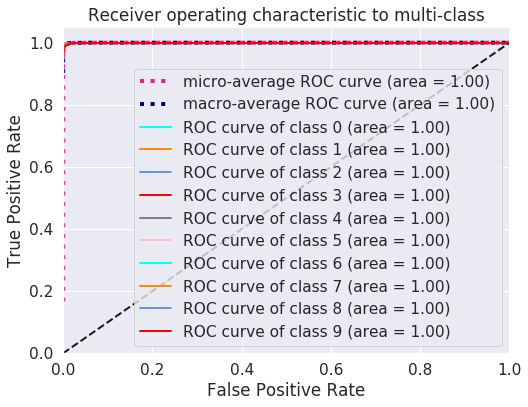
\includegraphics[width=0.8\textwidth]{thesis_template/images/roc.png}
    \caption{\small AUC-ROC graph of the model after 25 epochs}
    \label{}
    \end{figure}
    
\newpage \noindent Since it is a multi-class classifier it looks a bit hard to see all the curves but from the values represented on the right side shows that the value of ROC is always near 1.0 for all the classes which shows that the model is good. This explains that the AUC for all the classes is also 1.0. Since it is a multi-class classifier we also need micro and macro averaged ROC curves.  Micro and macro indicate slightly two different things. A macro average computes ROC independently for each class and then take the average, whereas micro average calculates the aggregate values together and then averages it. This helps us to find out if there is an imbalance in different classes. \\

\noindent Now let us take a look at feature maps for a particular image when passed through this model.



\begin{figure}[h]
    \centering
    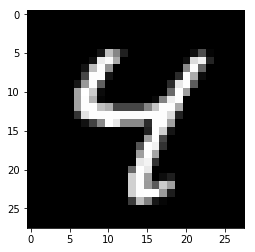
\includegraphics[width=0.4\textwidth]{thesis_template/images/4.png}
    \caption{\small Image 1 selected to visualize}
    \label{}
    \end{figure}


\begin{figure}[h!]
    \centering
    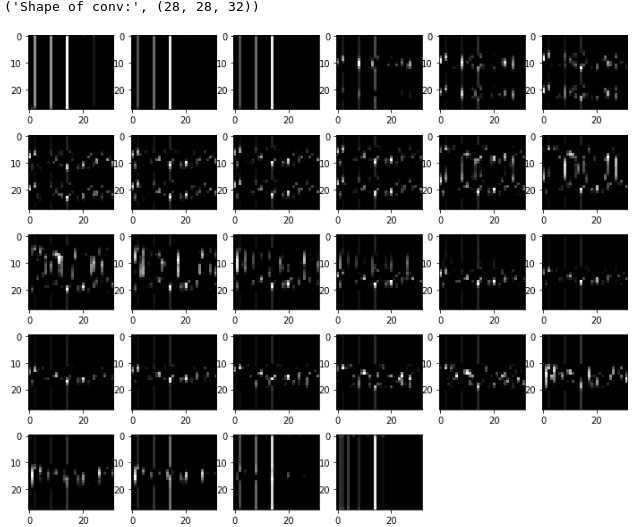
\includegraphics[width=1.0\textwidth]{thesis_template/images/filters.png}
    \caption{\small Filters of first activation layer for image 1}
    \label{}
    \end{figure}


\newpage \noindent  These are the 28 random activations in the first layer, as we can see the visualizations are not clear and it is hard to tell which pattern is recognized by the filters inside that layer. And there are some redundant filters as well for example the first three filters look the same it interprets that they recognize the same patterns. As per previous works the intermediate layers were supposed to recognize low level patterns but here these feature maps does not seem to recognize the patterns of input image. Now let us look at the second layer activations for the same image.


 \begin{figure}[h]
    \centering
    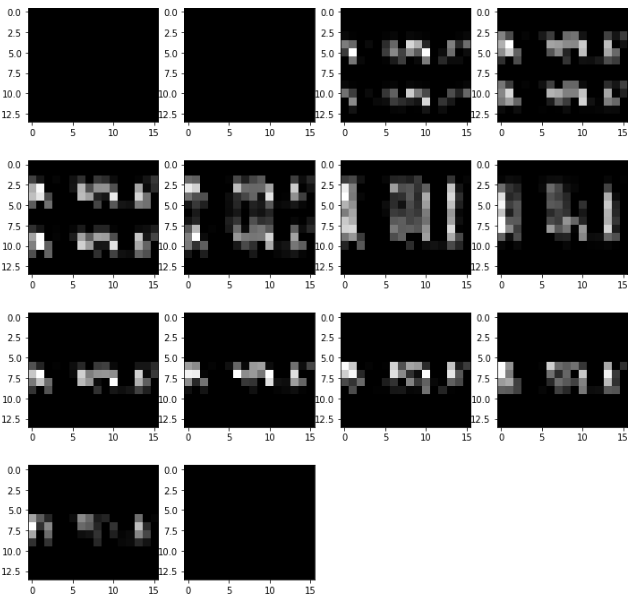
\includegraphics[width=1.0\textwidth]{thesis_template/images/layer2.png}
    \caption{\small Filters of second activation layer for image 1}
    \label{}
    \end{figure}

\newpage \noindent These are 14 random filters taken from the model after second convolution and activation. As per working mechanism of a convnet model the second layer activations depend on first layer so that is the reason why even these filters does not really depict anything. And as we can see there are three \textit{dead filters}. The blank images are considered as dead-filters because we can see that there is no pattern recognized and it looks completely blank. The filters also look very noisy which is a sign that network has not been trained long enough. \\
The third layer visualizations for the image also gave similar activations but just the shape was reduced because of the down sampling of image size. 




It could be the problem of image or the network might be biased for some images so let us look at the activations for another random image from the dataset. 


  \begin{figure}[h]
    \centering
    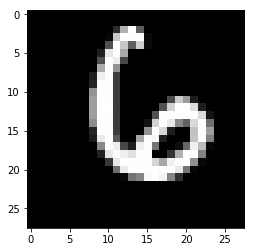
\includegraphics[width=0.5\textwidth]{thesis_template/images/6.png}
    \caption{\small Image 2 selected to visualize}
    \label{}
    \end{figure}
\newpage \noindent This image that belongs to different class and it was chosen randomly from test set. It generated the following visualizations after first activation.

\begin{figure}[h]
    \centering
    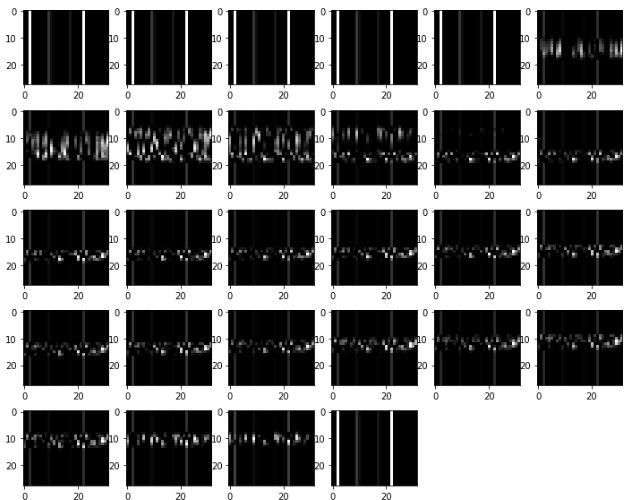
\includegraphics[width=0.8\textwidth]{thesis_template/images/6filers.png}
    \caption{\small First layer activations of image 2 }
    \label{}
    \end{figure}
    
\noindent The activations does not look like the patterns that are present in the input image. And most of the filters look similar it interprets the redundancy in the network. 

 \noindent PS: Even the second layer visualizations for the image looks similar to the first image that is the reason why they are not included here. It has 3 \textit{dead-filters}

\noindent Testing the same method on many different images from the test set showed similar activation filters. Not only this even the train images has shown few dead filters this show that the model has not converged properly and it cannot generalize well.

This indicates that though different performance metrics like accuracy, precision, recall are high there is a need to visualize filters. This is because the model described in the previous section has achieved an accuracy of 99.8\% but ended up with few dead-filters inside the network. In order achieve a model with good filters the model is modified slightly and trained it on more number of \textit{epochs} and less \textit{batch-size}.
\section{Upgraded Model}
In the previous section the model had \textit{Four Convolutional layers} each layer followed by \textit{Relu} and \textit{Max-pooling} layers. Here \textit{Batch-Normalization} layer is added after each Convolution layer and before Relu layer. According to \cite{Sergey} adding BN to the neural network helps us overcome problems with training the network and reduces the dependence of gradients on initial values. To increase the stability of networl BN normalizes the output of previous layer by substracting the batch mean and dividing batch standard deviation. It also makes sure that there is no activation that is either high nor low and thereby even the untrained parameters start to train. This could help us overcome more number of \textit{dead-filters} from the previous model. This model has following parameters.
\begin{itemize}
\item Dataset: MNIST
    \item Activation: Relu
    \item Optimizer: Adam
    \item Batch Normalization
    \item Filter-size: $3 \times 3$, Stride: 1, Padding: Zero
    \item Trained for 100 epochs 
    \item Batch-size: 32
    \item Number of filters remained same as previous model
    \item Dropout: 0.5\%
\end{itemize}

 \noindent Applying these parameters the model has achieved same accuracy of 99.8\%. The graph below represents the variation of accuracy and loss during training.
 \begin{figure}[h!]
    \centering
    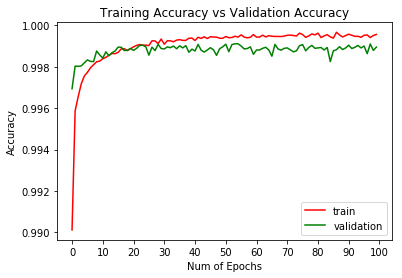
\includegraphics[width=0.8\textwidth]{thesis_template/images/100train.png}
    \caption{\small variation of accuracy during training}
    \label{}
    \end{figure}
\noindent As we can see both on train and validation datasets the accuracy had increased and decreased a bit but achieved maximum accuracy on both datasets.

 \begin{figure}[h!]
    \centering
    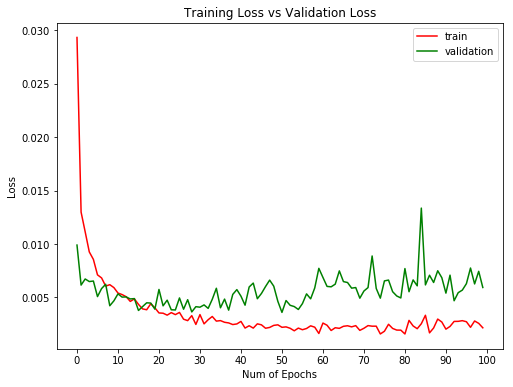
\includegraphics[width=0.8\textwidth]{thesis_template/images/100loss.png}
    \caption{\small variation of loss during training}
    \label{}
    \end{figure}
\newpage\noindent Here the loss on validation has variated more and the model has achieved loss of 0.004\%.

\begin{figure}[h!]
    \centering
    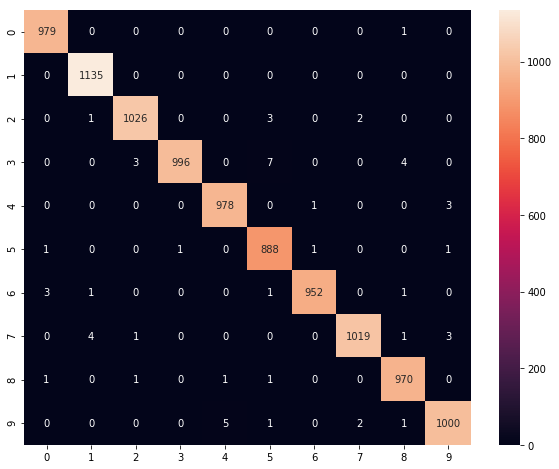
\includegraphics[width=0.85\textwidth]{thesis_template/images/con2.png}
    \caption{\small Confusion-matrix for modified model on test dataset}
    \label{}
    \end{figure}
\newpage\noindent Compared to confusion-matrix of previous model this model has a bit better classification of images. Because there are still images from each class that are misclassified. For example in the previous model and for "class 10" 18 images were predicted wrong, here 9 images were misclassified. This explains that parameters like batch-normalization and increasing epochs does not have much effect on entire performance of the model.
\begin{table}[h!]
\centering
\begin{tabular}{|l|l|l|l|l|}
\hline
          & precision & recall & f1-score & support \\ \hline
0         & 0.99      & 1.00   & 0.99     & 980     \\ \hline
1         & 0.99      & 1.00   & 1.00     & 1135    \\ \hline
2         & 1.00      & 0.99   & 0.99     & 1032    \\ \hline
3         & 0.99      & 1.00   & 0.99     & 1010    \\ \hline
4         & 0.99      & 1.00   & 0.99     & 982     \\ \hline
5         & 1.00      & 0.99   & 0.99     & 892     \\ \hline
6         & 0.99      & 0.99   & 0.99     & 958     \\ \hline
7         & 0.99      & 1.00   & 0.99     & 1028    \\ \hline
8         & 0.99      & 0.99   & 0.99     & 974     \\ \hline
9         & 1.00      & 0.99   & 0.99     & 1009    \\ \hline
avg/total & 0.99      & 0.99   & 0.99     & 10000   \\ \hline
\end{tabular}
\caption{Classification-report for upgraded model trained for 100 epochs on MNIST}
\end{table}
    
 \newpage\noindent The values of precision,recall and f1-score did not change much when compared to the previous model.\\   


\begin{figure}[h]
    \centering
    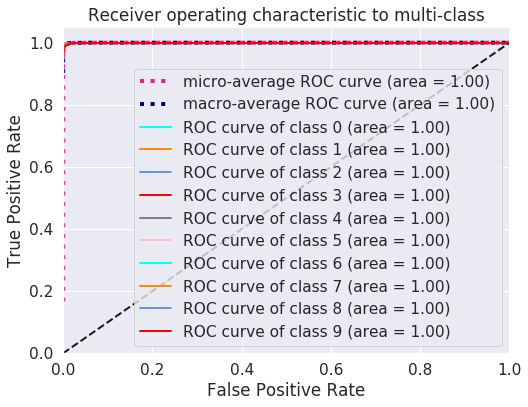
\includegraphics[width=0.6\textwidth]{thesis_template/images/roc.png}
    \caption{\small AUC-ROC curve for upgraded model trained for 100 epochs on MNIST}
    \label{}
    \end{figure}


\noindent Lastly, The AUC-ROC curve for both the models looks same. The AUC(Area Under Curve) for all the classes is 1 which indicates that the model is performing very well. Let us look at the visualizations of the upgraded model. 

\newpage\noindent Following image is selected from the test set

\begin{figure}[h!]
    \centering
    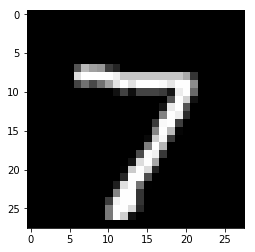
\includegraphics[width=0.3\textwidth]{thesis_template/images/7.png}
    \caption{\small Image 1 for Model 2}
    \label{}
    \end{figure}
 \noindent The image generated the following features in the first activation layer.   
    \begin{figure}[h!]
    \centering
    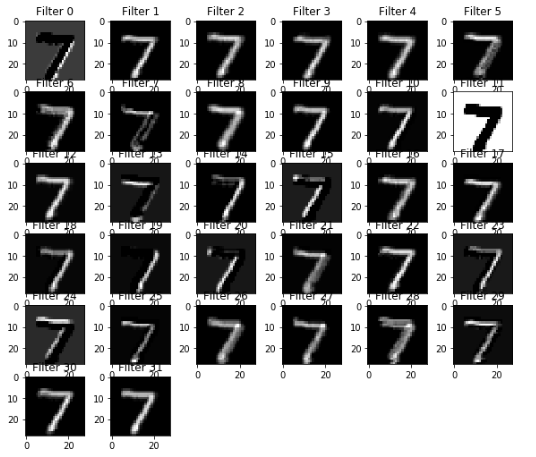
\includegraphics[width=0.9\textwidth]{thesis_template/images/71vis.png}
    \caption{\small First layer visualizations of model 2}
    \label{}
    \end{figure}

\newpage \noindent The first layer looks directly at the raw image pixels. At that stage, the activations are still retaining almost all of the information present in the initial picture. All the 32 filters are trained and there are no dead-filters. The activations are also more clear. Now let us see how the filters change as we go deeper in to the network.

    
\begin{figure}[h]
    \centering
    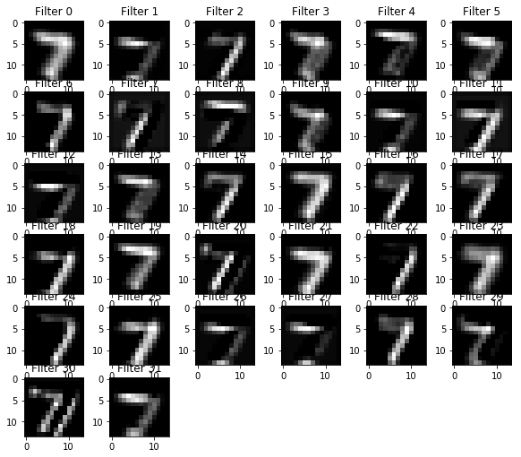
\includegraphics[width=1.0\textwidth]{thesis_template/images/72vis.png}
    \caption{\small Second layer visualizations of model 2}
    \label{}
    \end{figure}

\newpage \noindent The image represents the filters after second activation. All the filters are trained which is indication of no dead-filters. The white part inside each filter represents the pattern of the input image. We can notice that as we go deeper in to the model the filters look less like original image and has more abstract representation. Here all the filters are looking for almost similar type of patterns from input image. Let us see how there patterns are shared between 64 filters in the next convolution layer.


\begin{figure}[h]
    \centering
    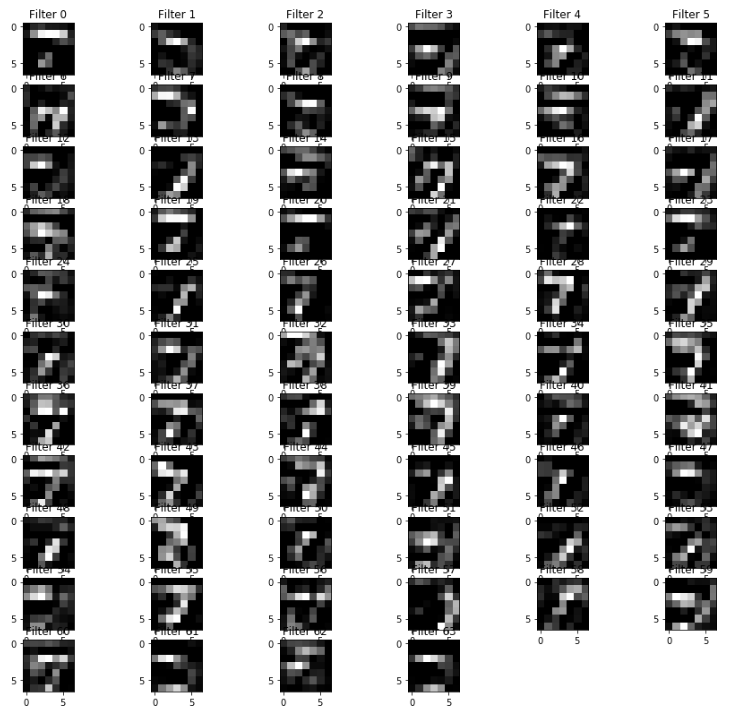
\includegraphics[width=0.95\textwidth]{thesis_template/images/73.png}
    \caption{\small Third layer visualizations of model 2}
    \label{}
    \end{figure}
 
 \newpage \noindent As we can see the filters in this layer are looking for variety of patterns from the input image. Now the difference can be seen as the presence of original image is much harder to see in these filters. It is a good indication that all the patterns are activated in different filters. For most of the features it is easy to say what part of image activated them. In order to show that the network is not biased one more image and its activations are shown here.
\begin{figure}[h]
    \centering
    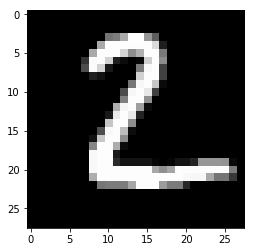
\includegraphics[width=0.5\textwidth]{thesis_template/images/2.png}
    \caption{\small Image 2}
    \label{}
    \end{figure}
\newpage The first three layer filters are shown below.
\begin{figure}[h!]
    \centering
    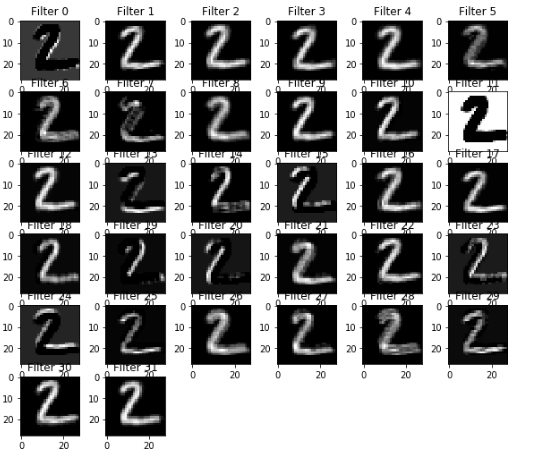
\includegraphics[width=0.95\textwidth]{thesis_template/images/21.png}
    \caption{\small first layer visualizations of model 2 for image 2}
    \label{}
    \end{figure}
    
\begin{figure}[h]
    \centering
    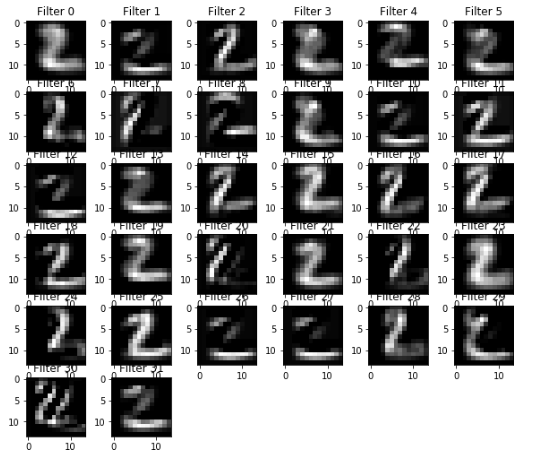
\includegraphics[width=1.0\textwidth]{thesis_template/images/22.png}
    \caption{\small Second layer visualizations of model 2 for image 2}
    \label{}
    \end{figure}
\newpage \noindent Both the layers does not contain any dead-filters. It is so clear that since the network has given 2 as input image most of the filters are activated in such a way that they produce high value for 2. Since the network is responsible to classify it as 2. It generates high outputs for 2s by having large weights aligned to pixels which tend to usually be high in images of 2s. Simultaneously, it can obtain relatively low outputs for non-2s by having small weights aligned to pixels which tend to be high in images of non-2s and low in images of 2s. One last thing is visualizing the third layer in the network.



\begin{figure}[h]
    \centering
    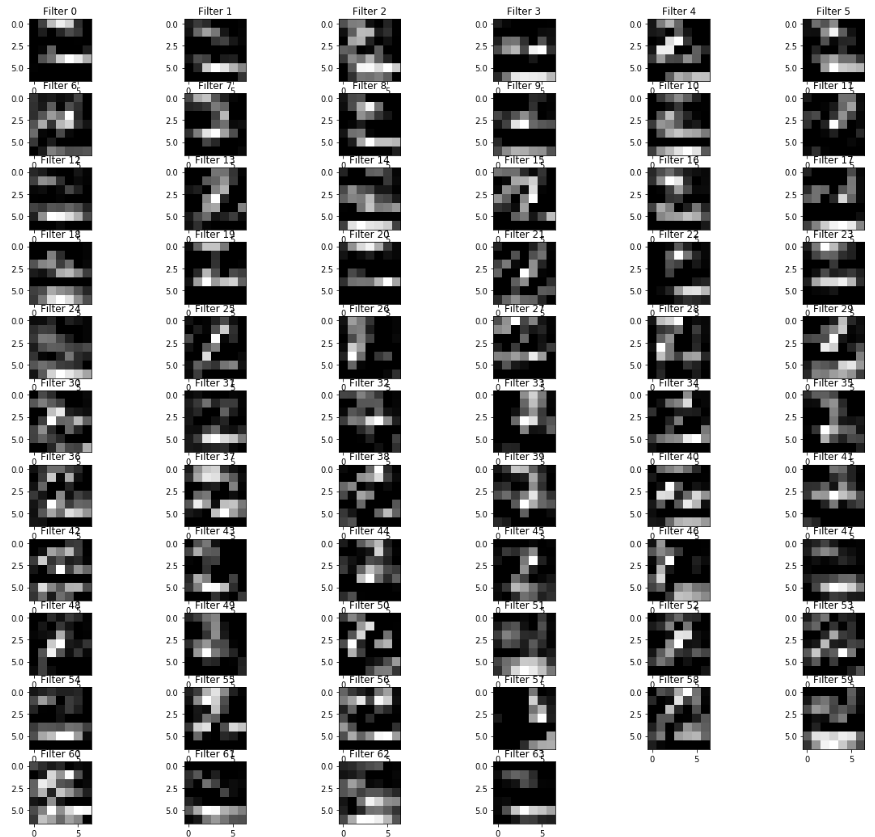
\includegraphics[width=0.9\textwidth]{thesis_template/images/23.png}
    \caption{\small Third layer visualizations of model 2 for image 2}
    \label{}
    \end{figure}
    
\newpage \noindent Some filters look like blurry 2. And the white part inside each filter represents the pixels of the input image that activate them. We can interpret these neurons as forming templates of output. The visualizations indicate that the network has converged. Till now we have seen the visualizations of network trained only on MNIST dataset which is very easy. Now let us look at the filters of the same network which is trained on CIFAR-10 dataset which has images of real world.

\newpage \section{Upgraded Model on CIFAR-10 dataset}
CIFAR-10 consists of 60000 labeled images which are of size $32 \times 32$ and have 3 channels. Here 50000 images belong to train dataset and 10000 belong to test dataset. And these images belong to 10 different classes which are airplanes, automobiles, birds, cats, deer, dogs, frogs, horses, ships, and trucks. The model is same with same parameters which are shown in upgraded model with batch-normalization layer. The model was trained for 100 epochs with batch-size of 32. The model has achieved the accuracy of 88\% on training dataset and loss of 0.3\%. On test dataset the accuracy achieved was 82\%.


\begin{figure}[h]
    \centering
    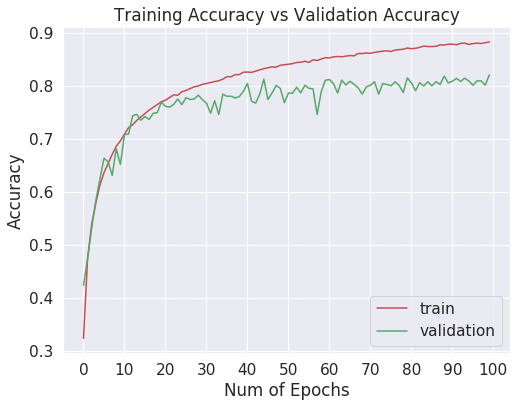
\includegraphics[width=0.52\textwidth]{thesis_template/images/cifacc.png}
    \caption{\small Variation of accuracy during training on CIFAR-10 for 100 epochs}
    \label{}
    \end{figure}

\begin{figure}[h]
    \centering
    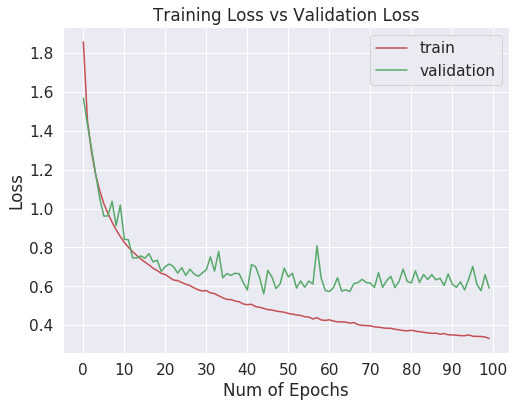
\includegraphics[width=0.52\textwidth]{thesis_template/images/cifloss.png}
    \caption{\small Variation of loss during training on CIFAR-10 for 100 epochs}
    \label{}
    \end{figure}
    
\begin{figure}[h]
    \centering
    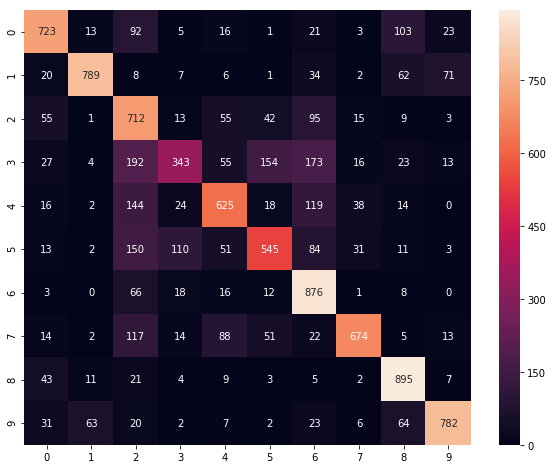
\includegraphics[width=0.7\textwidth]{thesis_template/images/cmcif.png}
    \caption{\small Confusion-matrix for CIFAR-10}
    \label{}
    \end{figure}
\newpage \noindent Here we can see that so many images are predicted wrong. Especially images that belong to class 3 seems to have more False Positives. The same model was unable to infer properly on other dataset. The precision, recall and f1-scores for the model are given below in Table 4.2. The values indicate that the model just has average performance.

\begin{table}[]
\centering
\begin{tabular}{|l|l|l|l|l|}
\hline
          & precision & recall & f1-score & support \\ \hline
0         & 0.77      & 0.72   & 0.74     & 1000     \\ \hline
1         & 0.89      & 0.79   & 0.84     & 1000    \\ \hline
2         & 0.47      & 0.71   & 0.56     & 1000    \\ \hline
3         & 0.64      & 0.35   & 0.45     & 1000    \\ \hline
4         & 0.67      & 0.62   & 0.65     & 1000    \\ \hline
5         & 0.66      & 0.55   & 0.60     & 1000     \\ \hline
6         & 0.60      & 0.88   & 0.71     & 1000     \\ \hline
7         & 0.86      & 0.67   & 0.75     & 1000   \\ \hline
8         & 0.75      & 0.90   & 0.82     & 1000     \\ \hline
9         & 0.85      & 0.78   & 0.82     & 1000    \\ \hline
avg/total & 0.72      & 0.70   & 0.69     & 10000   \\ \hline
\end{tabular}
\caption{Classification-report of upgraded model on CIFAR-10 after training for          100 epochs}
\end{table}

\newpage\begin{figure}[h]
    \centering
    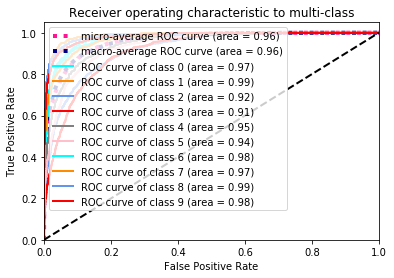
\includegraphics[width=0.68\textwidth]{thesis_template/images/cifroc.png}
    \caption{\small AUC $-$ ROC curve of CIFAR-10 after training for 100 epochs}
    \label{}
    \end{figure}

 \noindent Surprisingly the Area under curve indicates that the model has performed fine on the dataset. Now let us look at the images from the test dataset and the reaction of weights for that image. First image is horse  


\begin{figure}[h]
    \centering
    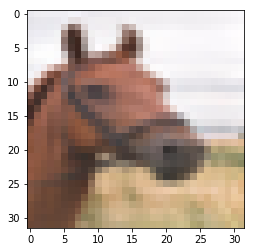
\includegraphics[width=0.45\textwidth]{thesis_template/images/horse.png}
    \caption{\small Horse image from CIFAR-10 }
    \label{}
    \end{figure}
    
\begin{figure}[h]
    \centering
    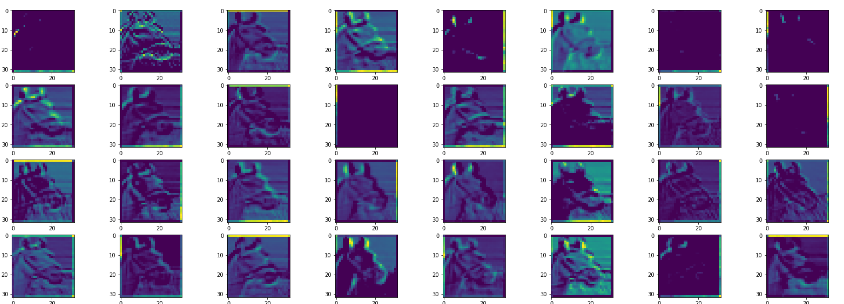
\includegraphics[width=1.0\textwidth]{thesis_template/images/horsefil1.png}
    \caption{\small 32 Filters of layer1}
    \label{}
    \end{figure}

\newpage \noindent All the features represent the input image. As we can see all the filters are activated and more patterns from the input image are seen. Next is second layer visualizations for this image.

\begin{figure}[h]
    \centering
    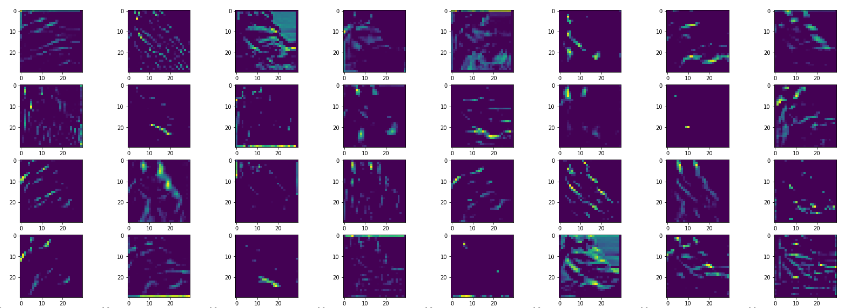
\includegraphics[width=1.1\textwidth]{thesis_template/images/horsefil2.png}
    \caption{\small 32 Filters of layer 2}
    \label{}
    \end{figure}
\newpage \noindent The figure represents the feature maps of layer 2. We can see that the patterns from the input image are less visible but still we can say which patterns activated particular filter. There are no dead-filters in both the layers. Next we will see how third layer visualizations look like.

\begin{figure}[h]
    \centering
    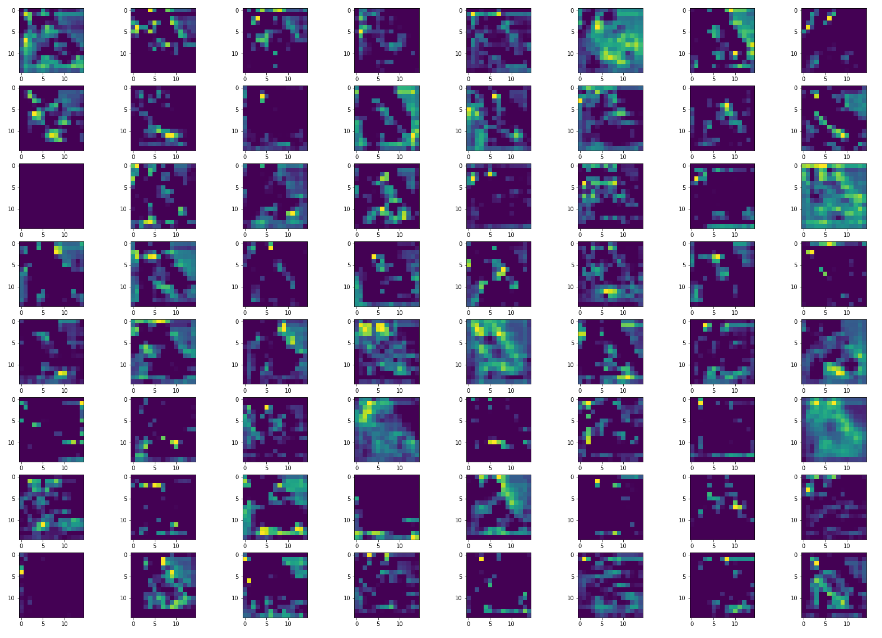
\includegraphics[width=1.0\textwidth]{thesis_template/images/horsefil3.png}
    \caption{\small 64 Filters of layer 3}
    \label{}
    \end{figure}
\newpage \noindent The figure represents all the 64 features from the third layer. It is hard to say which pattern activated the particular filter. The deeper layers encode higher-level features like nose,ears etc that is the reason why these feature maps contain less information about the input image. One more image from the cifar-10 is represented below.


\begin{figure}[h]
    \centering
    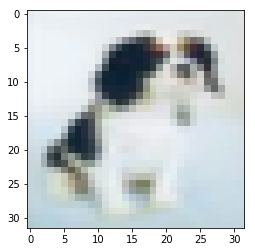
\includegraphics[width=0.45\textwidth]{thesis_template/images/dog1.png}
    \caption{\small Dog image from cifar-10}
    \label{}
    \end{figure}

\newpage\noindent The first layer activations for this image are\\
\begin{figure}[h]
    \centering
    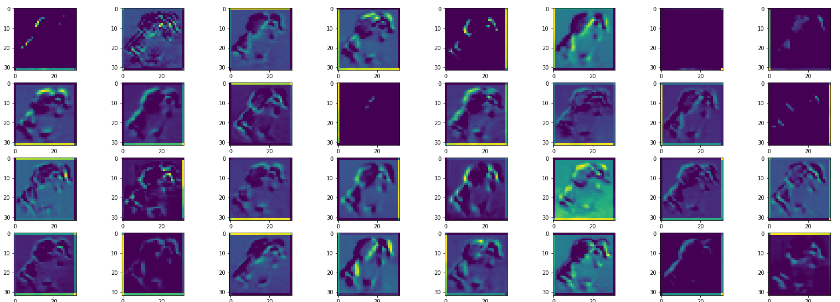
\includegraphics[width=1.1\textwidth]{thesis_template/images/dog1fil1.png}
    \caption{\small 32 Filters of layer 1 for image 2}
    \label{}
    \end{figure}\\
\noindent For both the images taken from cifar-10 dataset in the layer 3 , 17th filter does not activate at all which indicates the dead-filter. But here there is only one dead-filter so this can ignored. The filters of second and third layer for the dog image are shown in the next page.   

\begin{figure}[h]
    \centering
    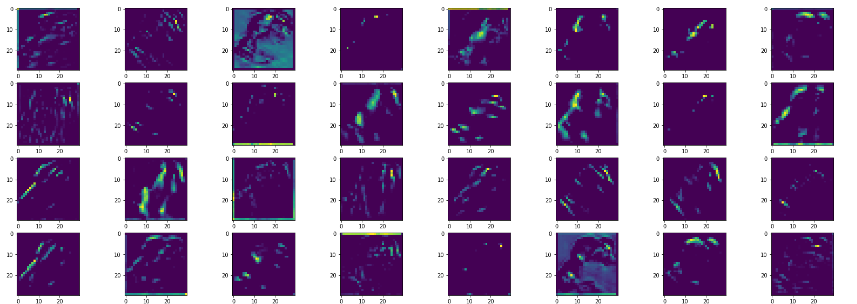
\includegraphics[width=1.0\textwidth]{thesis_template/images/dog1fil2.png}
    \caption{\small 32 Filters of layer 2 for image 2}
    \label{}
    \end{figure}


\begin{figure}[h]
    \centering
    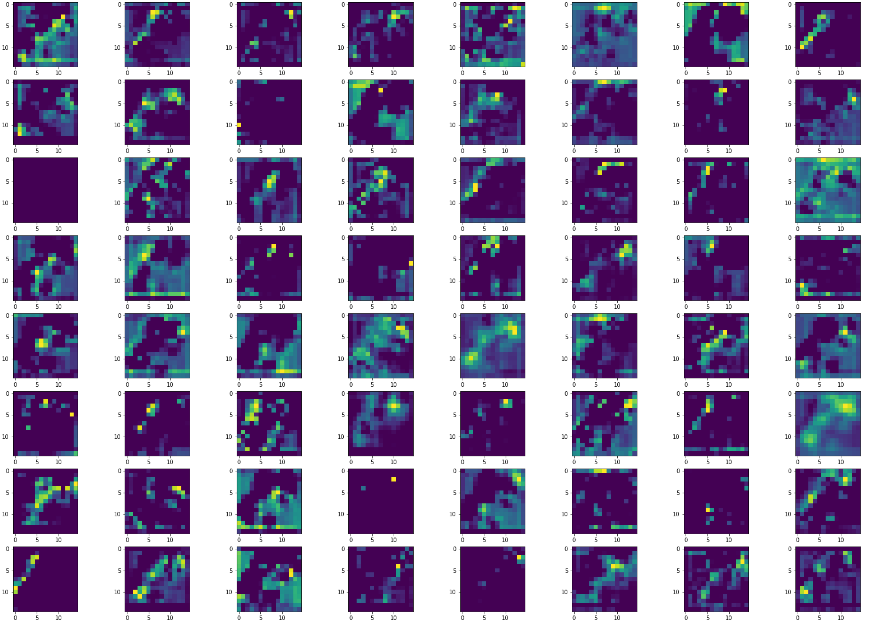
\includegraphics[width=1.0\textwidth]{thesis_template/images/dog1fil3.png}
    \caption{\small 64 Filters of layer 3 for image 2}
    \label{}
    \end{figure}
